\documentclass[10pt,aspectratio=169]{beamer}

\usetheme{Madrid}
\usecolortheme{default}
\usefonttheme{professionalfonts}

\setbeamertemplate{navigation symbols}{}
\setbeamertemplate{footline}[frame number]
\setbeamercolor{block title}{bg=blue!20,fg=black}
\setbeamercolor{block body}{bg=blue!5,fg=black}

\usepackage[utf8]{inputenc}
\usepackage{amsmath}
\usepackage{booktabs}
\usepackage{array}
\usepackage{tikz}
\usetikzlibrary{arrows.meta,positioning}

\title[MyHealthReport V1]{MyHealthReport}
\subtitle{Version 1 Framework}
\author{}
\date{22 August 2026}

\begin{document}

\begin{frame}
\titlepage
\end{frame}

\begin{frame}{Agenda}
\tableofcontents
\end{frame}

% =========================================================
\section{Purpose \& Principles}
% =========================================================

\begin{frame}{1. Purpose of Version 1}
MyHealthReport Version 1 is a \textbf{structured health interpretation and wellness-navigation platform}. It helps a user to:
\begin{columns}[T]
\begin{column}{0.5\textwidth}
\begin{enumerate}
\item Understand their basic health profile
\item Upload and structure a blood test report
\item Identify out-of-range lab values
\item Understand patterns between results
\item Answer only relevant questions
\end{enumerate}
\end{column}
\begin{column}{0.5\textwidth}
\begin{enumerate}\setcounter{enumi}{5}
\item Route findings: wellness vs. medical review
\item Receive a short, prioritised action plan
\item Understand the reasoning behind it
\item Track results over time
\end{enumerate}
\end{column}
\end{columns}
\vfill
\begin{alertblock}{Not a diagnostic tool}
Version 1 should \textbf{not} attempt to diagnose disease independently.
\end{alertblock}
\end{frame}

\begin{frame}{Central Logic}
\begin{center}
\Large
Data $\rightarrow$ Abnormality $\rightarrow$ Pattern $\rightarrow$ Context $\rightarrow$ Safety \\[4pt]
$\rightarrow$ Priority $\rightarrow$ Action $\rightarrow$ Explanation $\rightarrow$ Follow-up
\end{center}
\end{frame}

\begin{frame}{2. Core Design Principles}
\begin{block}{1. Start simple}
Registration collects only what's useful across almost every analysis; detailed questions come later, triggered by findings.
\end{block}
\begin{block}{2. Never interpret one number in isolation}
Result + Reference Range + Related Markers + Patient Profile + Symptoms + History + Trend
\end{block}
\begin{block}{3. Safety overrides wellness advice}
A clinically significant finding triggers medical assessment first; wellness advice becomes secondary.
\end{block}
\end{frame}

\begin{frame}{2. Core Design Principles (cont.)}
\begin{block}{4. Explain the reasoning}
Every recommendation answers: \textbf{What did we find? Why might it matter? What can you do? Why should that help?}
\end{block}
\begin{block}{5. Prioritise instead of overwhelming}
Twenty abnormal values should not produce twenty recommendations --- group related abnormalities and surface the upstream priorities.
\end{block}
\end{frame}

% =========================================================
\section{System Architecture}
% =========================================================

\begin{frame}{3. Version 1 System Architecture}
\centering
\scriptsize
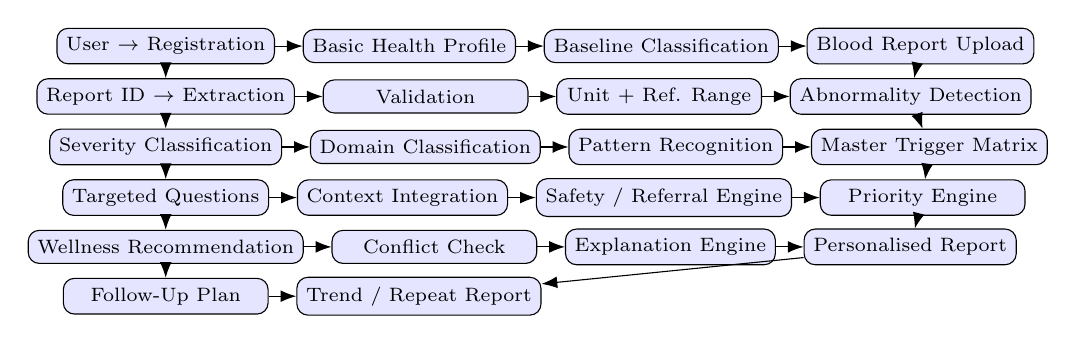
\begin{tikzpicture}[
  node distance=5pt and 10pt,
  box/.style={draw, rounded corners, fill=blue!10, minimum width=2.6cm, minimum height=0.42cm, align=center, font=\scriptsize},
  arr/.style={-{Latex[length=2mm]}}
]
\node[box] (n1) {User $\to$ Registration};
\node[box, right=of n1] (n2) {Basic Health Profile};
\node[box, right=of n2] (n3) {Baseline Classification};
\node[box, right=of n3] (n4) {Blood Report Upload};

\node[box, below=of n1] (n5) {Report ID $\to$ Extraction};
\node[box, right=of n5] (n6) {Validation};
\node[box, right=of n6] (n7) {Unit + Ref. Range};
\node[box, right=of n7] (n8) {Abnormality Detection};

\node[box, below=of n5] (n9) {Severity Classification};
\node[box, right=of n9] (n10) {Domain Classification};
\node[box, right=of n10] (n11) {Pattern Recognition};
\node[box, right=of n11] (n12) {Master Trigger Matrix};

\node[box, below=of n9] (n13) {Targeted Questions};
\node[box, right=of n13] (n14) {Context Integration};
\node[box, right=of n14] (n15) {Safety / Referral Engine};
\node[box, right=of n15] (n16) {Priority Engine};

\node[box, below=of n13] (n17) {Wellness Recommendation};
\node[box, right=of n17] (n18) {Conflict Check};
\node[box, right=of n18] (n19) {Explanation Engine};
\node[box, right=of n19] (n20) {Personalised Report};

\node[box, below=of n17] (n21) {Follow-Up Plan};
\node[box, right=of n21] (n22) {Trend / Repeat Report};

\draw[arr] (n1)--(n2); \draw[arr] (n2)--(n3); \draw[arr] (n3)--(n4);
\draw[arr] (n4)--(n8); \draw[arr] (n5)--(n6); \draw[arr] (n6)--(n7); \draw[arr] (n7)--(n8);
\draw[arr] (n8)--(n12); \draw[arr] (n9)--(n10); \draw[arr] (n10)--(n11); \draw[arr] (n11)--(n12);
\draw[arr] (n12)--(n16); \draw[arr] (n13)--(n14); \draw[arr] (n14)--(n15); \draw[arr] (n15)--(n16);
\draw[arr] (n16)--(n20); \draw[arr] (n17)--(n18); \draw[arr] (n18)--(n19); \draw[arr] (n19)--(n20);
\draw[arr] (n20)--(n22); \draw[arr] (n21)--(n22);
\draw[arr] (n1)--(n5); \draw[arr] (n5)--(n9); \draw[arr] (n9)--(n13); \draw[arr] (n13)--(n17); \draw[arr] (n17)--(n21);
\end{tikzpicture}
\end{frame}

% =========================================================
\section{Module 1--3: Profile, Intake, Validation}
% =========================================================

\begin{frame}{4. Module 1: Basic Health Profile}
\textbf{Objective:} enough baseline information to interpret future blood tests without a burdensome registration.
\vspace{4pt}
\scriptsize
\begin{columns}[T]
\begin{column}{0.5\textwidth}
\begin{itemize}
\item Age / date of birth
\item Biological sex
\item Height, weight, waist circumference
\item Blood pressure, if known
\end{itemize}
\end{column}
\begin{column}{0.5\textwidth}
\begin{itemize}
\item Smoking status, alcohol use
\item General physical activity
\item Known major medical conditions
\item Regular medication; pregnancy status
\end{itemize}
\end{column}
\end{columns}
\vfill
\begin{exampleblock}{Automatically calculated}
$$BMI = \dfrac{Weight\,(kg)}{Height\,(m)^2}$$ \quad then classify weight status.
\end{exampleblock}
\end{frame}

\begin{frame}{5. Module 2: Blood Report Intake}
\textbf{Objective:} convert a laboratory report into structured data.
\vspace{6pt}

\textbf{Step 1 --- Identify Report:} lab name, report date, patient identifiers, units, reference ranges.

\vspace{8pt}
\textbf{Step 2 --- Extract Results} (structured record):
\scriptsize
\begin{center}
\begin{tabular}{ll}
\toprule
Field & Example \\
\midrule
Test & ALT \\
Result & 65 \\
Unit & U/L \\
Reference range & 0--40 \\
Lab flag & High \\
Report date / source & 22 Aug 2026 / Laboratory A \\
\bottomrule
\end{tabular}
\end{center}
\end{frame}

\begin{frame}{6. Module 3: Data Validation}
Before interpretation, the system checks:
\begin{itemize}
\item Was the value extracted correctly?
\item Does the unit make sense? Is the reference range available?
\item Is the test name recognised? Is the result biologically plausible?
\item Are there duplicates? Is a previous result available?
\end{itemize}
\vfill
\begin{alertblock}{If confidence is low: user confirmation required}
\footnotesize ``We detected potassium 8.4 mmol/L. Please confirm that this value was read correctly from your report.''
\end{alertblock}
This prevents extraction errors from becoming health advice.
\end{frame}

% =========================================================
\section{Module 4--7: Ranges, Domains, Severity}
% =========================================================

\begin{frame}{7. Module 4: Reference Range Architecture}
Every laboratory marker carries \textbf{three layers}:
\begin{block}{Layer A --- Laboratory Reference Interval}
Taken directly from the uploaded report, preserved exactly (e.g. ALT: 0--40 U/L).
\end{block}
\begin{block}{Layer B --- Clinical Decision Threshold}
Recognised guideline thresholds, which may differ from the lab's population range.
\end{block}
\begin{block}{Layer C --- Platform Interpretation Rule}
$$Relative\ Elevation = \dfrac{Result}{Upper\ Limit\ of\ Normal}$$
e.g. ALT 80 / ULN 40 = 2$\times$ ULN --- comparable across labs.
\end{block}
\end{frame}

\begin{frame}{8. Module 5: Laboratory Domain Classification}
\scriptsize
\begin{columns}[T]
\begin{column}{0.5\textwidth}
\begin{itemize}
\item \textbf{A. Full Blood Count} --- Hb, RBC, Hct, MCV, MCH, MCHC, RDW, WBC, differential, platelets
\item \textbf{B. Glucose / Metabolic} --- fasting glucose, HbA1c
\item \textbf{C. Lipid Profile} --- total cholesterol, LDL-C, HDL-C, triglycerides, non-HDL
\item \textbf{D. Liver} --- ALT, AST, ALP, GGT, bilirubin, albumin, total protein
\end{itemize}
\end{column}
\begin{column}{0.5\textwidth}
\begin{itemize}
\item \textbf{E. Kidney} --- creatinine, eGFR, urea, sodium, potassium
\item \textbf{F. Uric Acid}
\item \textbf{G. Thyroid} --- TSH, free T4, free T3
\item \textbf{H. Iron / Nutritional} --- ferritin, iron, transferrin, TIBC, B12, folate, vitamin D
\end{itemize}
\end{column}
\end{columns}
\vfill
\normalsize Version 1 focuses on common panels rather than every possible test.
\end{frame}

\begin{frame}{9. Module 6: Abnormality Detection}
\textbf{Basic status:} Normal / Low / High
\vspace{6pt}
\begin{center}
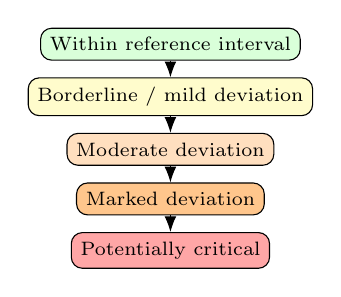
\begin{tikzpicture}[node distance=6pt, every node/.style={font=\scriptsize}]
\node[draw,rounded corners,fill=green!15] (a) {Within reference interval};
\node[draw,rounded corners,fill=yellow!20,below=of a] (b) {Borderline / mild deviation};
\node[draw,rounded corners,fill=orange!25,below=of b] (c) {Moderate deviation};
\node[draw,rounded corners,fill=orange!45,below=of c] (d) {Marked deviation};
\node[draw,rounded corners,fill=red!35,below=of d] (e) {Potentially critical};
\draw[-{Latex[length=2mm]}] (a)--(b); \draw[-{Latex[length=2mm]}] (b)--(c);
\draw[-{Latex[length=2mm]}] (c)--(d); \draw[-{Latex[length=2mm]}] (d)--(e);
\end{tikzpicture}
\end{center}
\vfill
Thresholds are marker-specific --- not all ``slightly outside range'' values carry equal importance.
\end{frame}

\begin{frame}{10. Module 7: Severity Framework --- Six Action Levels}
\scriptsize
\begin{center}
\begin{tabular}{@{}p{1.6cm}p{9.8cm}@{}}
\toprule
\textbf{Level} & \textbf{Meaning} \\
\midrule
0 & Within expected range --- no major concern \\
1 & Optimisation opportunity --- not abnormal, but room to improve \\
2 & Mild abnormality --- lifestyle review, monitoring, follow-up \\
3 & Clinically relevant --- may warrant clinician assessment \\
4 & High-risk finding --- medical assessment prioritised \\
5 & Potential critical finding --- urgent safety pathway activated \\
\bottomrule
\end{tabular}
\end{center}
\end{frame}

% =========================================================
\section{Module 8--10: Patterns \& Questions}
% =========================================================

\begin{frame}{11. Module 8: Pattern Recognition Engine}
The system looks for \textbf{combinations}, not isolated values.
\begin{exampleblock}{Metabolic Pattern}
\scriptsize BMI$\uparrow$, waist$\uparrow$, triglycerides$\uparrow$, HDL$\downarrow$, glucose/HbA1c$\uparrow$, BP$\uparrow$, ALT$\uparrow$ $\Rightarrow$ \textit{Metabolic-risk pattern} (not a diagnosis)
\end{exampleblock}
\begin{exampleblock}{Microcytic Pattern}
\scriptsize Hb$\downarrow$, MCV$\downarrow$, MCH$\downarrow$ $\Rightarrow$ ferritin/iron studies, blood loss \& dietary history, referral logic
\end{exampleblock}
\begin{exampleblock}{Liver Pattern}
\scriptsize ALT/AST-predominant vs. ALP/GGT-predominant $\Rightarrow$ different question sets
\end{exampleblock}
\end{frame}

\begin{frame}{12. Module 9: Master Trigger Matrix}
\begin{center}
\small
LAB FINDING $\rightarrow$ PATTERN $\rightarrow$ TRIGGER $\rightarrow$ TARGETED QUESTION SET
\end{center}
\vspace{6pt}
\scriptsize
\begin{center}
\begin{tabular}{ll}
\toprule
Trigger & Question \\
\midrule
ALT elevated & Alcohol intake / Medication / Supplements \\
ALT elevated & Known fatty liver / Recent heavy exercise \\
ALT + metabolic markers abnormal & Weight change \\
GGT elevated & Alcohol context \\
Significant abnormality & Relevant symptoms \\
\bottomrule
\end{tabular}
\end{center}
The patient answers only the questions that matter to their results.
\end{frame}

\begin{frame}{13. Module 10: Targeted Question Engine}
\scriptsize
\begin{columns}[T]
\begin{column}{0.5\textwidth}
\begin{itemize}
\item \textbf{Symptoms} --- fatigue, dizziness, chest discomfort, breathlessness, jaundice, bleeding, severe weakness
\item \textbf{Medical History} --- diabetes, hypertension, kidney/liver/thyroid/cardiovascular disease
\item \textbf{Medication} --- regular, recent, supplements, herbal products
\end{itemize}
\end{column}
\begin{column}{0.5\textwidth}
\begin{itemize}
\item \textbf{Diet} --- targeted, e.g. triglycerides high $\to$ sugary drinks, refined carbs, alcohol, overeating
\item \textbf{Exercise} --- frequency, duration, intensity, resistance work, sedentary time
\item \textbf{Sleep} --- duration, quality, irregularity, sleep-disordered breathing
\item \textbf{Stress} --- low / moderate / high + major stressors
\end{itemize}
\end{column}
\end{columns}
\end{frame}

% =========================================================
\section{Module 11--14: Context, Safety, Priority}
% =========================================================

\begin{frame}{14. Module 11: Context Integration Engine}
\begin{center}
\large
LAB RESULTS + PATIENT PROFILE + MEDICAL HISTORY \\[4pt]
+ MEDICATIONS + SYMPTOMS + LIFESTYLE + PREVIOUS RESULTS
\end{center}
\vfill
\centering This creates the health context used by later engines.
\end{frame}

\begin{frame}{15. Module 12: Safety and Referral Engine}
\textbf{Main question:} Is this situation appropriate for routine wellness guidance?
\vspace{8pt}
\begin{columns}[T]
\begin{column}{0.48\textwidth}
\begin{block}{If YES}
Routine Wellness Pathway --- no major safety concern identified.
\end{block}
\end{column}
\begin{column}{0.48\textwidth}
\begin{alertblock}{If NO --- escalate}
\scriptsize Medical Review Recommended $\to$ Prompt Medical Assessment $\to$ Urgent Assessment
\end{alertblock}
\end{column}
\end{columns}
\vfill
\footnotesize Exact clinical thresholds are built separately in the \textbf{Safety Matrix} and medically validated before implementation.
\end{frame}

\begin{frame}{16. Module 13: Priority Engine}
\footnotesize Example patient: obesity, elevated BP, high triglycerides, elevated glucose, mild ALT elevation, high uric acid --- instead of six separate recommendations:
\vspace{6pt}
\begin{enumerate}
\item \textbf{Priority 1:} Metabolic health / weight management
\item \textbf{Priority 2:} Blood pressure
\item \textbf{Priority 3:} Cardiovascular risk
\item \textbf{Priority 4:} Liver monitoring
\end{enumerate}
\vfill
This makes the action plan easier to follow.
\end{frame}

\begin{frame}{17. Module 14: Root-Factor Mapping}
\centering
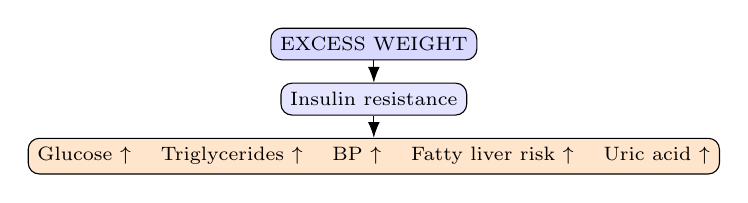
\begin{tikzpicture}[node distance=8pt, every node/.style={font=\scriptsize}]
\node[draw,rounded corners,fill=blue!15] (w) {EXCESS WEIGHT};
\node[draw,rounded corners,fill=blue!10,below=of w] (ir) {Insulin resistance};
\node[draw,rounded corners,fill=orange!20,below=of ir] (g) {Glucose $\uparrow$ \quad Triglycerides $\uparrow$ \quad BP $\uparrow$ \quad Fatty liver risk $\uparrow$ \quad Uric acid $\uparrow$};
\draw[-{Latex[length=2mm]}] (w)--(ir); \draw[-{Latex[length=2mm]}] (ir)--(g);
\end{tikzpicture}
\vfill
\raggedright \footnotesize \textit{``Weight management is prioritised because it may positively influence several current metabolic findings at the same time.''}
\end{frame}

% =========================================================
\section{Module 15--18: Recommendations \& Explanation}
% =========================================================

\begin{frame}{18. Module 15: Wellness Recommendation Engine}
Version 1 recommendations focus on:
\begin{columns}[T]
\begin{column}{0.5\textwidth}
\begin{itemize}
\item Nutrition
\item Physical activity
\item Weight management
\item Sleep
\end{itemize}
\end{column}
\begin{column}{0.5\textwidth}
\begin{itemize}
\item Stress management
\item Smoking cessation / alcohol moderation
\item Hydration where appropriate
\item General preventive health behaviour
\end{itemize}
\end{column}
\end{columns}
\vfill
Advice should be proportional to the evidence available.
\end{frame}

\begin{frame}{19. Recommendation Structure}
\scriptsize
TRIGGER $\to$ HEALTH ISSUE $\to$ RECOMMENDATION $\to$ WHY $\to$ EXPECTED BENEFIT $\to$ PRECAUTION $\to$ FOLLOW-UP
\vspace{6pt}
\begin{exampleblock}{Example}
\scriptsize
\textbf{Trigger:} Elevated triglycerides + excess body weight \\
\textbf{Recommendation:} Reduce refined carbs and sugary beverages; gradual weight reduction \\
\textbf{Why:} Excess energy / refined-carb intake contributes to elevated triglycerides \\
\textbf{Expected Benefit:} Improved triglycerides and broader metabolic health \\
\textbf{Precaution:} May need modification per medical conditions, medication, nutrition status \\
\textbf{Follow-Up:} Repeat relevant measurements per clinical plan
\end{exampleblock}
\end{frame}

\begin{frame}{20. Module 16: Recommendation Conflict Resolver}
All recommendations pass a safety filter before being shown.
\vspace{6pt}
\scriptsize
\begin{center}
\begin{tabular}{p{3.6cm}p{3.6cm}p{3.6cm}}
\toprule
Recommendation & Conflict & Action \\
\midrule
Increase exercise intensity & Severe anaemia / cardiac symptoms & Do not issue routine intensive advice \\
High-protein diet & Kidney impairment & Modify or suppress pending assessment \\
Aggressive weight loss & Pregnancy / underweight & Suppress recommendation \\
\bottomrule
\end{tabular}
\end{center}
\end{frame}

\begin{frame}{21. Module 17: Recommendation Priority System}
Each recommendation is scored on:
\begin{itemize}
\item Clinical importance \quad \textbullet\ Modifiability
\item Number of findings affected \quad \textbullet\ Safety
\item Expected health benefit \quad \textbullet\ User feasibility
\end{itemize}
\vfill
\begin{alertblock}{Target output}
Approximately \textbf{3 main priorities}, with secondary recommendations underneath. Avoid ten equally-weighted actions.
\end{alertblock}
\end{frame}

\begin{frame}{22. Module 18: Explanation Engine}
Every important recommendation offers:
\scriptsize
\begin{itemize}
\item \textbf{What we found} --- ``Your triglyceride level is above the laboratory reference range.''
\item \textbf{Why it may matter} --- ``Elevated triglycerides can be associated with metabolic and cardiovascular risk.''
\item \textbf{What may contribute} --- excess weight, dietary pattern, alcohol, glucose regulation, inactivity
\item \textbf{What you can do} --- specific actions
\item \textbf{Why this may help} --- mechanistic explanation
\item \textbf{What happens next} --- monitoring, repeat testing, or professional assessment
\end{itemize}
\end{frame}

% =========================================================
\section{Report, Tracking \& Data Model}
% =========================================================

\begin{frame}{23. Module 19: Final User Report Structure}
\scriptsize
\begin{enumerate}
\item \textbf{Health Snapshot} --- BMI, BP category, smoking status, activity level, baseline risks
\item \textbf{Laboratory Overview} --- Within range / Needs attention / Higher priority / Medical review recommended
\item \textbf{Key Patterns} --- e.g. metabolic-risk, iron-related, liver enzyme abnormality
\item \textbf{Your Top Priorities} --- usually three
\item \textbf{Recommended Actions} --- concrete, measurable
\item \textbf{Why These Actions Matter} --- causal reasoning
\item \textbf{Medical Follow-Up} --- separate from wellness advice
\item \textbf{Monitoring Plan} --- weight, waist, BP, activity, labs, symptoms
\end{enumerate}
\end{frame}

\begin{frame}{24. Module 20: Longitudinal Tracking}
\begin{columns}[T]
\begin{column}{0.45\textwidth}
\small
\begin{tabular}{lr}
\toprule
Date & HbA1c \\
\midrule
Jan & 5.6 \\
Apr & 5.8 \\
Aug & 6.1 \\
\bottomrule
\end{tabular}
\end{column}
\begin{column}{0.55\textwidth}
\small
Instead of ``HbA1c is elevated,'' the system can say: \textit{``Your HbA1c has shown a progressive upward trend across three measurements.''}
\vspace{8pt}
\textbf{Trend categories:} Improving, Stable, Worsening, Fluctuating
\end{column}
\end{columns}
\end{frame}

\begin{frame}{25. Version 1 Database Concept}
\scriptsize
Core structured objects (not free text):
\begin{columns}[T]
\begin{column}{0.33\textwidth}
\begin{itemize}
\item Patient
\item Laboratory Report
\item Laboratory Result
\item Health Domain
\item Trigger
\end{itemize}
\end{column}
\begin{column}{0.33\textwidth}
\begin{itemize}
\item Question
\item Answer
\item Pattern
\item Safety Rule
\item Recommendation
\end{itemize}
\end{column}
\begin{column}{0.33\textwidth}
\begin{itemize}
\item Contraindication
\item Priority
\item Explanation
\item Follow-Up
\end{itemize}
\end{column}
\end{columns}
\end{frame}

\begin{frame}[fragile]{26. Master Rule Architecture}
\scriptsize
\begin{verbatim}
IF Finding X AND/OR Finding Y AND Patient Context Z
THEN Activate Question Set A
THEN Assess Safety Rule B
THEN Identify Pattern C
THEN Generate Recommendation D
UNLESS Contraindication E
THEN Assign Priority F AND Generate Explanation G
AND Generate Follow-Up H
\end{verbatim}
\normalsize
The standard structure for almost every clinical/wellness rule in the platform.
\end{frame}

% =========================================================
\section{AI Role, Scope \& Roadmap}
% =========================================================

\begin{frame}{27--28. The Role of AI}
\begin{columns}[T]
\begin{column}{0.5\textwidth}
\begin{block}{AI \textbf{should} do}
\scriptsize
\begin{itemize}
\item Report extraction assistance
\item Natural-language explanation
\item Summarisation \& personalised wording
\item Identifying relevant rules
\item Explaining relationships between findings
\item Generating patient-friendly reports
\end{itemize}
\end{block}
\end{column}
\begin{column}{0.5\textwidth}
\begin{alertblock}{AI should \textbf{not} independently control}
\scriptsize
\begin{itemize}
\item Emergency triggers, critical thresholds
\item Contraindications, referral criteria
\item Diagnostic claims
\item Medication advice
\item Clinically sensitive recommendations
\end{itemize}
\end{alertblock}
\end{column}
\end{columns}
\vfill
\centering \footnotesize \textit{Structured clinical rules determine what is allowed. AI determines how it is explained.}
\end{frame}

\begin{frame}{29. Version 1 Scope Boundary}
\scriptsize
\begin{columns}[T]
\begin{column}{0.5\textwidth}
\begin{exampleblock}{Include}
Basic profile, BMI, BP context, common blood tests, abnormality detection, severity classification, common pattern recognition, targeted questions, wellness recommendations, red-flag/referral logic, explanations, trend tracking, report generation
\end{exampleblock}
\end{column}
\begin{column}{0.5\textwidth}
\begin{alertblock}{Delay to later versions}
Supplement marketplace, automatic supplement prescribing, pharmacy sales integration, complex genetic interpretation, imaging interpretation, diagnosis engine, medication initiation/adjustment, complex specialist disease management, autonomous AI clinical decisions
\end{alertblock}
\end{column}
\end{columns}
\end{frame}

\begin{frame}{30. Clinical Domains --- Build Order}
\begin{enumerate}
\item \textbf{Phase 1 --- Metabolic / cardiovascular:} BMI, BP, glucose, HbA1c, lipid profile \\
\footnotesize \textit{strong preventive-health foundation} \normalsize
\item \textbf{Phase 2 --- Liver + kidney}
\item \textbf{Phase 3 --- Full blood count + iron}
\item \textbf{Phase 4 --- Thyroid + uric acid + nutritional markers}
\end{enumerate}
\vfill
Do not attempt to build every laboratory module simultaneously.
\end{frame}

\begin{frame}{31. The Four Master Matrices}
\scriptsize
\begin{columns}[T]
\begin{column}{0.5\textwidth}
\textbf{A. Laboratory Interpretation Matrix} \\
Marker, Reference logic, Severity, Related markers, Potential patterns
\vspace{8pt}
\textbf{B. Trigger Question Matrix} \\
Finding, Trigger, Question, Why, Possible responses
\end{column}
\begin{column}{0.5\textwidth}
\textbf{C. Safety / Referral Matrix} \\
Finding, Threshold/combination, Risk level, Action, Referral urgency
\vspace{8pt}
\textbf{D. Recommendation Matrix} \\
Finding/pattern, Recommendation, Why, Contraindications, Priority, Follow-up
\end{column}
\end{columns}
\vfill
\centering These four matrices are the \textbf{brain of MyHealthReport}.
\end{frame}

\begin{frame}{32. Version 1 Decision Flow}
\centering
\scriptsize
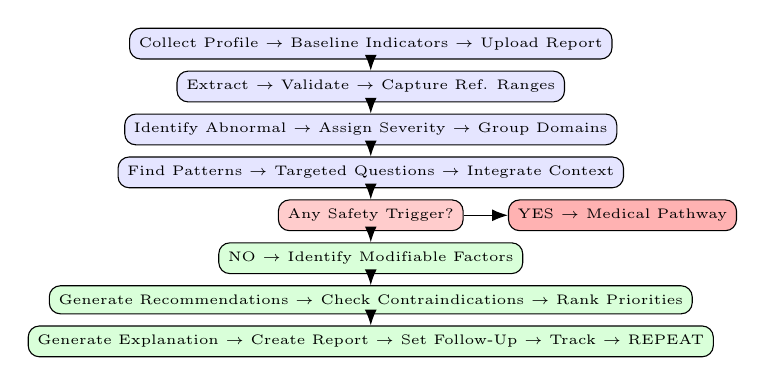
\begin{tikzpicture}[node distance=4pt, every node/.style={font=\tiny}]
\node[draw,rounded corners,fill=blue!10] (a) {Collect Profile $\to$ Baseline Indicators $\to$ Upload Report};
\node[draw,rounded corners,fill=blue!10,below=of a] (b) {Extract $\to$ Validate $\to$ Capture Ref. Ranges};
\node[draw,rounded corners,fill=blue!10,below=of b] (c) {Identify Abnormal $\to$ Assign Severity $\to$ Group Domains};
\node[draw,rounded corners,fill=blue!10,below=of c] (d) {Find Patterns $\to$ Targeted Questions $\to$ Integrate Context};
\node[draw,rounded corners,fill=red!20,below=of d] (e) {Any Safety Trigger?};
\node[draw,rounded corners,fill=red!30,right=16pt of e] (f) {YES $\to$ Medical Pathway};
\node[draw,rounded corners,fill=green!15,below=of e] (g) {NO $\to$ Identify Modifiable Factors};
\node[draw,rounded corners,fill=green!15,below=of g] (h) {Generate Recommendations $\to$ Check Contraindications $\to$ Rank Priorities};
\node[draw,rounded corners,fill=green!15,below=of h] (i) {Generate Explanation $\to$ Create Report $\to$ Set Follow-Up $\to$ Track $\to$ REPEAT};
\draw[-{Latex[length=2mm]}] (a)--(b); \draw[-{Latex[length=2mm]}] (b)--(c); \draw[-{Latex[length=2mm]}] (c)--(d);
\draw[-{Latex[length=2mm]}] (d)--(e); \draw[-{Latex[length=2mm]}] (e)--(f); \draw[-{Latex[length=2mm]}] (e)--(g);
\draw[-{Latex[length=2mm]}] (g)--(h); \draw[-{Latex[length=2mm]}] (h)--(i);
\end{tikzpicture}
\end{frame}

% =========================================================
\section{Identity \& Master Algorithm}
% =========================================================

\begin{frame}{33. The Identity of MyHealthReport}
\begin{center}
\small \textit{Not:} ``AI tells you what your blood test means.''

\vspace{6pt}
\large \textbf{But:} ``MyHealthReport turns your blood results, health profile\\ and lifestyle into a personalised health roadmap.''
\end{center}
\vspace{10pt}
\begin{center}
\begin{tabular}{cccccc}
\textbf{Understand} & \textbf{Prioritise} & \textbf{Act} & \textbf{Escalate} & \textbf{Explain} & \textbf{Track}
\end{tabular}
\end{center}
\end{frame}

\begin{frame}{34. The Central MyHealthReport Algorithm}
$$Health\ Interpretation = Lab\ Findings + Patterns + Patient\ Context + Risk + Trend$$
\vspace{4pt}
$$Action\ Plan = Priority \times Modifiability \times Benefit \times Safety$$
\vspace{4pt}
\begin{center}
\textit{subject to}
\end{center}
$$Safety\ Override > Wellness\ Recommendation$$
\vspace{4pt}
$$MyHealthReport = Understand + Prioritise + Act + Explain + Monitor$$
\vfill
\footnotesize \centering This is the Version 1 master architecture. The next layer is the \textbf{Master Clinical Logic System}: Laboratory Interpretation, Trigger, Safety, and Recommendation Matrices.
\end{frame}

\begin{frame}
\centering
\Huge Thank You
\vspace{10pt}

\normalsize \textit{MyHealthReport --- Version 1 Framework}
\end{frame}

\end{document}
